\chapter{Results}

\shorthandoff{-} 

\section{Výběr presumptivních pseudomonád}
Na základě výsledků primárních biochemických testů a~popisu morfologie buněk a~kolonií dle~standardů České sbírky mikroorganismů bylo vytypováno 439 presumptivních kmenů pseudomonád.
Jednalo se o vzorky izolované z Antarktidy pořízené během výprav české expedice v letech 2011 až 2014 na stanici Johanna Gregora Mendela, jenž byla vybudována na ostrově Jamese Rosse.
Z~roku~2011 bylo takto vytypováno 194~kmenů, z~roku~2012 se~jednalo o~43~kmenů, 116~kmenů bylo vybráno z~roku~2013 a~86~z~roku~2014.
Soubor vybraných kmenů z~let 2011 a~2012 obsahoval mimo abiotické vzorky (půda, voda) též výtěry z~tlamy a~rekta tuleňů.

\section{Selekce \tax{Pseudomonas} spp.}
\begin{figure}[h!!!]
  \centering
  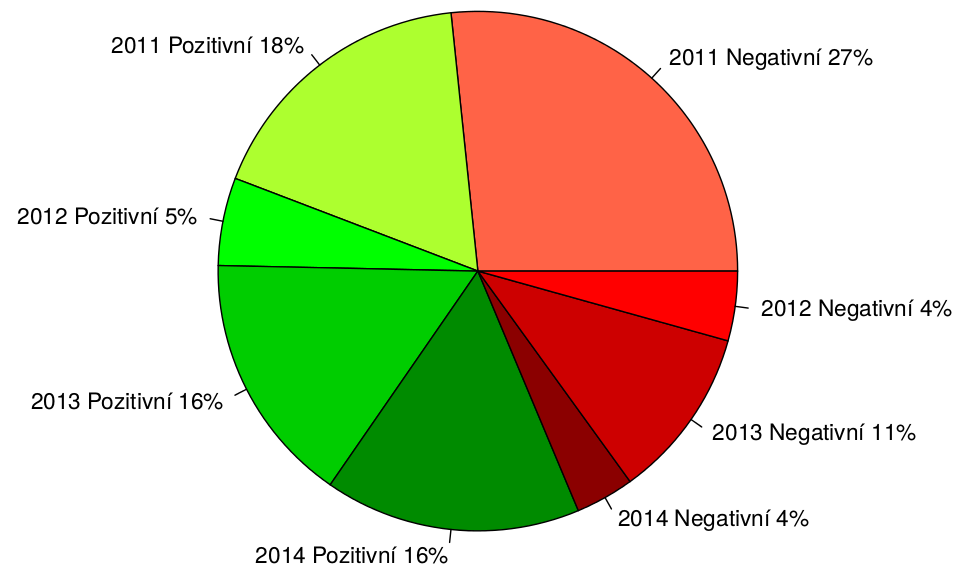
\includegraphics[scale=0.31]{text/Pictures/Graf_PCR_Poz-Neg.png}
	\caption{Výsledky selekce pseudomonád rodově specifickými PCR z jednotlivých let}
	\label{PCR_P-N}
\end{figure}
Pro potvrzení předběžného rodového zařazení \tax{Pseudomonas} spp. v~souboru presumptivních pseudomonád byly vybrány 2 jednoduché, rodově specifické PCR.
Z~celkových 439~kmenů jsem pomocí alespoň jedné PCR detekovala amplikon o~specifické délce u~240~izolátů.
Podrobnější zastoupení pozitivních a negativních kmenů v rámci jednotlivých let si lze prohlédnout na~Obrázku~\ref{PCR_P-N}.
Zelené výseče odpovídají pozitivním, červené negativním reakcím.

Takto detekovaných 240 kmenů, spadajících dle alespoň jedné z~použitých PCR do~rodu \tax{Pseudomonas}, bylo podrobeno další fenotypizaci a genotypizaci.

\section{Fenotypizace}
\subsection{Základní charakteristika}
Jedná se o gramnegativní krátké tyčky s podobnou morfologií.
Většina izolátů tvoří krémové či béžové kolonie s hladkým povrchem, souvislým okrajem a mírně vypouklým středem.
Avšak u 19 kmenů byla pozorována produkce nažloutlého, u kmenů P3865 a~P5916 žlutého a u P3765 a P4206 dokonce oranžového pigmentu.
Kmeny P3866, P3894 a~P4277 se přitom vyznačují tvorbou hnědého exopigmentu.

Co se týče růstové teploty, jde převážně o psychrotrofy, jelikož zhruba 90 \% kultur roste v~rozmezí 5 až 30$^\circ$C.
Osm kmenů však nebylo schopno růstu při 5$^\circ$C.
Jako psychrofilní lze označit pouze 21 izolátů, jelikož nevykazují růst již při 30 $^\circ$C a jejich teplotní maximum pro~růst se bude pohybovat okolo 20$^\circ$C.
Velmi úzké teplotní rozmezí bylo pozorováno u~vzorků P3765, P4876, P4885 a P5180, které nerostly jak při 30$^\circ$C, tak ani při~5$^\circ$C.
Zato u~celkem 8 kmenů můžeme pozorovat růst v rozmezí 5 až 37$^\circ$C.
Všichni zástupci rostou při~15$^\circ$C.


\subsection{Biochemická aktivita}
\subsubsection{Výsledy testů předcházejících výběru presumptivních pseudomonád}
Všechny izolované kmeny z Antarktidy byly podrobeny základní sadě konvenčních biochemických a fyziologických testů dle standardů České sbírky mikroorganismů.
Mezi~kandidáty s biochemickou aktivitou připomínající \tax{Pseudomonas} spp. bylo vybráno 439~kmenů.
Všichni takto vytypovaní zástupci spadali mezi gramnegativní glukózu nefermentující tyčky.
Kromě neschopnosti fermentace glukózy patřily mezi klíčové znaky pro~výběr také produkce katalázy, přítomnost fluorescence na~King~B mediu, redukce nitrátů a nitritů, dekarboxylace aminokyselin a hydrolýza eskulinu.

Z celkového počtu 240 kmenů, následně zařazených dle výsledků jednoduchých PCR do~rodu \tax{Pseudomonas}, jen necelých 56\% produkuje fluorescentní pigment na~mediu King~B.
74~izolátů redukuje nitráty, přičemž 27 z nich za současné produkce plynu.
Nitrity redukuje pouze 63 pseudomonád, avšak P4108, P4815, P4850, P4860, P4884 a~P5434 takto činí bez~schopnosti předchozí redukce nitrátů na nitrity.
Čtrnáct zástupců hydrolyzuje eskulin, třicet dekarboxyluje lyzin a čtyři ornitin.
Zato arginin je degradován téměř 75ti~procenty testovaných vzorků.\\



\shorthandon{-} 
%%%%%%%%%%%%%%%%%%%%%%%%%%%%%%%%%%%%


\cleardoublepage

